\documentclass{siamltex}

%% ----------------------------------------------------------------------
%% Packages
%% ----------------------------------------------------------------------
\usepackage{amsmath,amsfonts,amssymb}
\usepackage[usenames]{color}

%% For \boldsymbol
\usepackage{amsbsy}

%% For \bm (bold math)
\usepackage{bm}

%% For proper spacing in text macros
\usepackage{xspace}

%% For special lists like inparaenum, compactenum, compactitem
\usepackage{paralist}

%% Do fun things with tabular environment
\usepackage{array}

%% Graphics
\usepackage{graphicx}
\DeclareGraphicsExtensions{.png}

%% For \subfloat command
\usepackage{subfig}

%% For hyperlinks. Should always be the last package.
\usepackage[colorlinks,urlcolor=blue,citecolor=blue,linkcolor=blue]{hyperref}

%% Show labels
\usepackage[notref,notcite]{showkeys}

%% Algorithm
\usepackage{algorithm}
\usepackage{algpseudocode}

%% ----------------------------------------------------------------------
%% Theorem-like envirnoments
%% ----------------------------------------------------------------------

% Property
\newtheorem{claim}[theorem]{Claim}
\newtheorem{fact}[theorem]{Fact}
\newtheorem{obs}[theorem]{Observation}
\newtheorem{defn}[theorem]{Definition}
\newtheorem{observation}[theorem]{Observation}
\newtheorem{property}[theorem]{Property}

% Example - but take away italicized characters by wrapping another environment around it.
\newtheorem{example_hidden}[theorem]{Example}
\newenvironment{example}{\begin{example_hidden}\rm}{~~$\square$\end{example_hidden}}

%% ----------------------------------------------------------------------
%% Definitions
%% ----------------------------------------------------------------------

%% Useful shorthand for converting equations to be inline
\newenvironment{inlinemath}{$}{$}

%% Shorthand for Real and Complex
\newcommand{\Real}{\mathbb{R}}
\newcommand{\Natural}{\mathbb{N}}
\newcommand{\Complex}{\mathbb{C}}

%%% BOLDFACE LETTERS
\newcommand{\bG}{{\bf G}}
\newcommand{\bT}{{\bf T}}

%%% CALLIGRAPHIC LETTERS
\newcommand{\cA}{{\cal A}}
\newcommand{\cB}{{\cal B}}
\newcommand{\cC}{{\cal C}}
\newcommand{\cD}{{\cal D}}
\newcommand{\cE}{{\cal E}}
\newcommand{\cF}{{\cal F}}
\newcommand{\cG}{{\cal G}}
\newcommand{\cH}{{\cal H}}
\newcommand{\cI}{{\cal I}}
\newcommand{\cJ}{{\cal J}}
\newcommand{\cL}{{\cal L}}
\newcommand{\cM}{{\cal M}}
\newcommand{\cP}{{\cal P}}
\newcommand{\cR}{{\cal R}}
\newcommand{\cS}{{\cal S}}
\newcommand{\cT}{{\cal T}}
\newcommand{\cU}{{\cal U}}
\newcommand{\cV}{{\cal V}}

%% Miscellaneous math stuff

\newcommand{\lin}[2]{Line(#1^{(#2)})}
\newcommand{\move}[3]{#1^{(#2:#3)}}
\newcommand{\bdim}{dim}
\newcommand{\cyl}{cyl}
\newcommand{\pr}{{\rm Pr}}
\newcommand{\poly}{\textrm{poly}}
\newcommand{\p}{\mathcal{P}}
\newcommand{\mymod}{\textrm{mod} \ }
\newcommand{\otilde}{\widetilde{O}}
\newcommand{\qed}{\hfill $\Box$}
\newcommand{\eps}{\varepsilon}
\newcommand{\fu}{\varphi}
\newcommand{\restr}[1]{{|_{{\textstyle #1}}}}
\newcommand{\proj}{\mbox{\rm proj}}
\newcommand{\vol}{\mbox{\tt vol}\,}
\newcommand{\area}{\mbox{\tt area}\,}
\newcommand{\conv}{\mbox{\tt conv}\,}
\newcommand{\diam}{\hbox{\tt diam}\,}
\newcommand{\hdisc}{\mbox{\rm herdisc}}
\newcommand{\ldisc}{\mbox{\rm lindisc}}
\newcommand{\EX}{\hbox{\bf E}}
\newcommand{\prob}{{\rm Prob}}
\newcommand{\proofend}{{\medskip\medskip}}
\newcommand{\reals}{{\rm I\!\hspace{-0.025em} R}}
\newcommand{\dist}{\hbox{dist}}
\newcommand{\defeq}{\mbox{\,$\stackrel{\rm def}{=}$\,}}


%% Hyper-linked References
\newcommand{\Sec}[1]{\hyperref[sec:#1]{\S\ref*{sec:#1}}} %section
\newcommand{\Eqn}[1]{\hyperref[eq:#1]{(\ref*{eq:#1})}} %equation
\newcommand{\Fig}[1]{\hyperref[fig:#1]{Figure~\ref*{fig:#1}}} %figure
\newcommand{\Tab}[1]{\hyperref[tab:#1]{Table~\ref*{tab:#1}}} %table
\newcommand{\Thm}[1]{\hyperref[thm:#1]{Theorem~\ref*{thm:#1}}} %theorem
\newcommand{\Lem}[1]{\hyperref[lem:#1]{Lemma~\ref*{lem:#1}}} %lemma
\newcommand{\Prop}[1]{\hyperref[prop:#1]{Property~\ref*{prop:#1}}} %property
\newcommand{\Cor}[1]{\hyperref[cor:#1]{Corollary~\ref*{cor:#1}}} %corollary
\newcommand{\Def}[1]{\hyperref[def:#1]{Definition~\ref*{def:#1}}} %definition
\newcommand{\Alg}[1]{\hyperref[alg:#1]{Algorithm~\ref*{alg:#1}}} %algorithm
\newcommand{\Ex}[1]{\hyperref[ex:#1]{Example~\ref*{ex:#1}}} %example

%% Comments to ourselves
\newcommand{\Reminder}[1]{{\color{red}#1}}

%% Useful formatting commands
\newcommand{\V}[1]{{\bm{\mathbf{\MakeLowercase{#1}}}}} % vector
\newcommand{\M}[1]{{\bm{\mathbf{\MakeUppercase{#1}}}}} % matrix
\newcommand{\qtext}[1]{\quad\text{#1}\quad} % text with quads around it


%% ----------------------------------------------------------------------
%% Begin Document
%% ----------------------------------------------------------------------

\begin{document}

%% ----------------------------------------------------------------------
%% Frontmatter
%% ----------------------------------------------------------------------

\title{ 5-Vertex patterns
}\author{Ali Pinar\footnotemark[2] }
\maketitle

\centerline {\sc \today}

\renewcommand{\thefootnote}{\fnsymbol{footnote}}
%\footnotetext[2]{Sandia National Laboratories, Livermore, CA. Email: \{tgkolda,apinar,scomand\}@sandia.gov.}
\renewcommand{\thefootnote}{\arabic{footnote}}
\section{Introduction} 

\begin{figure}[h]
\begin{center}
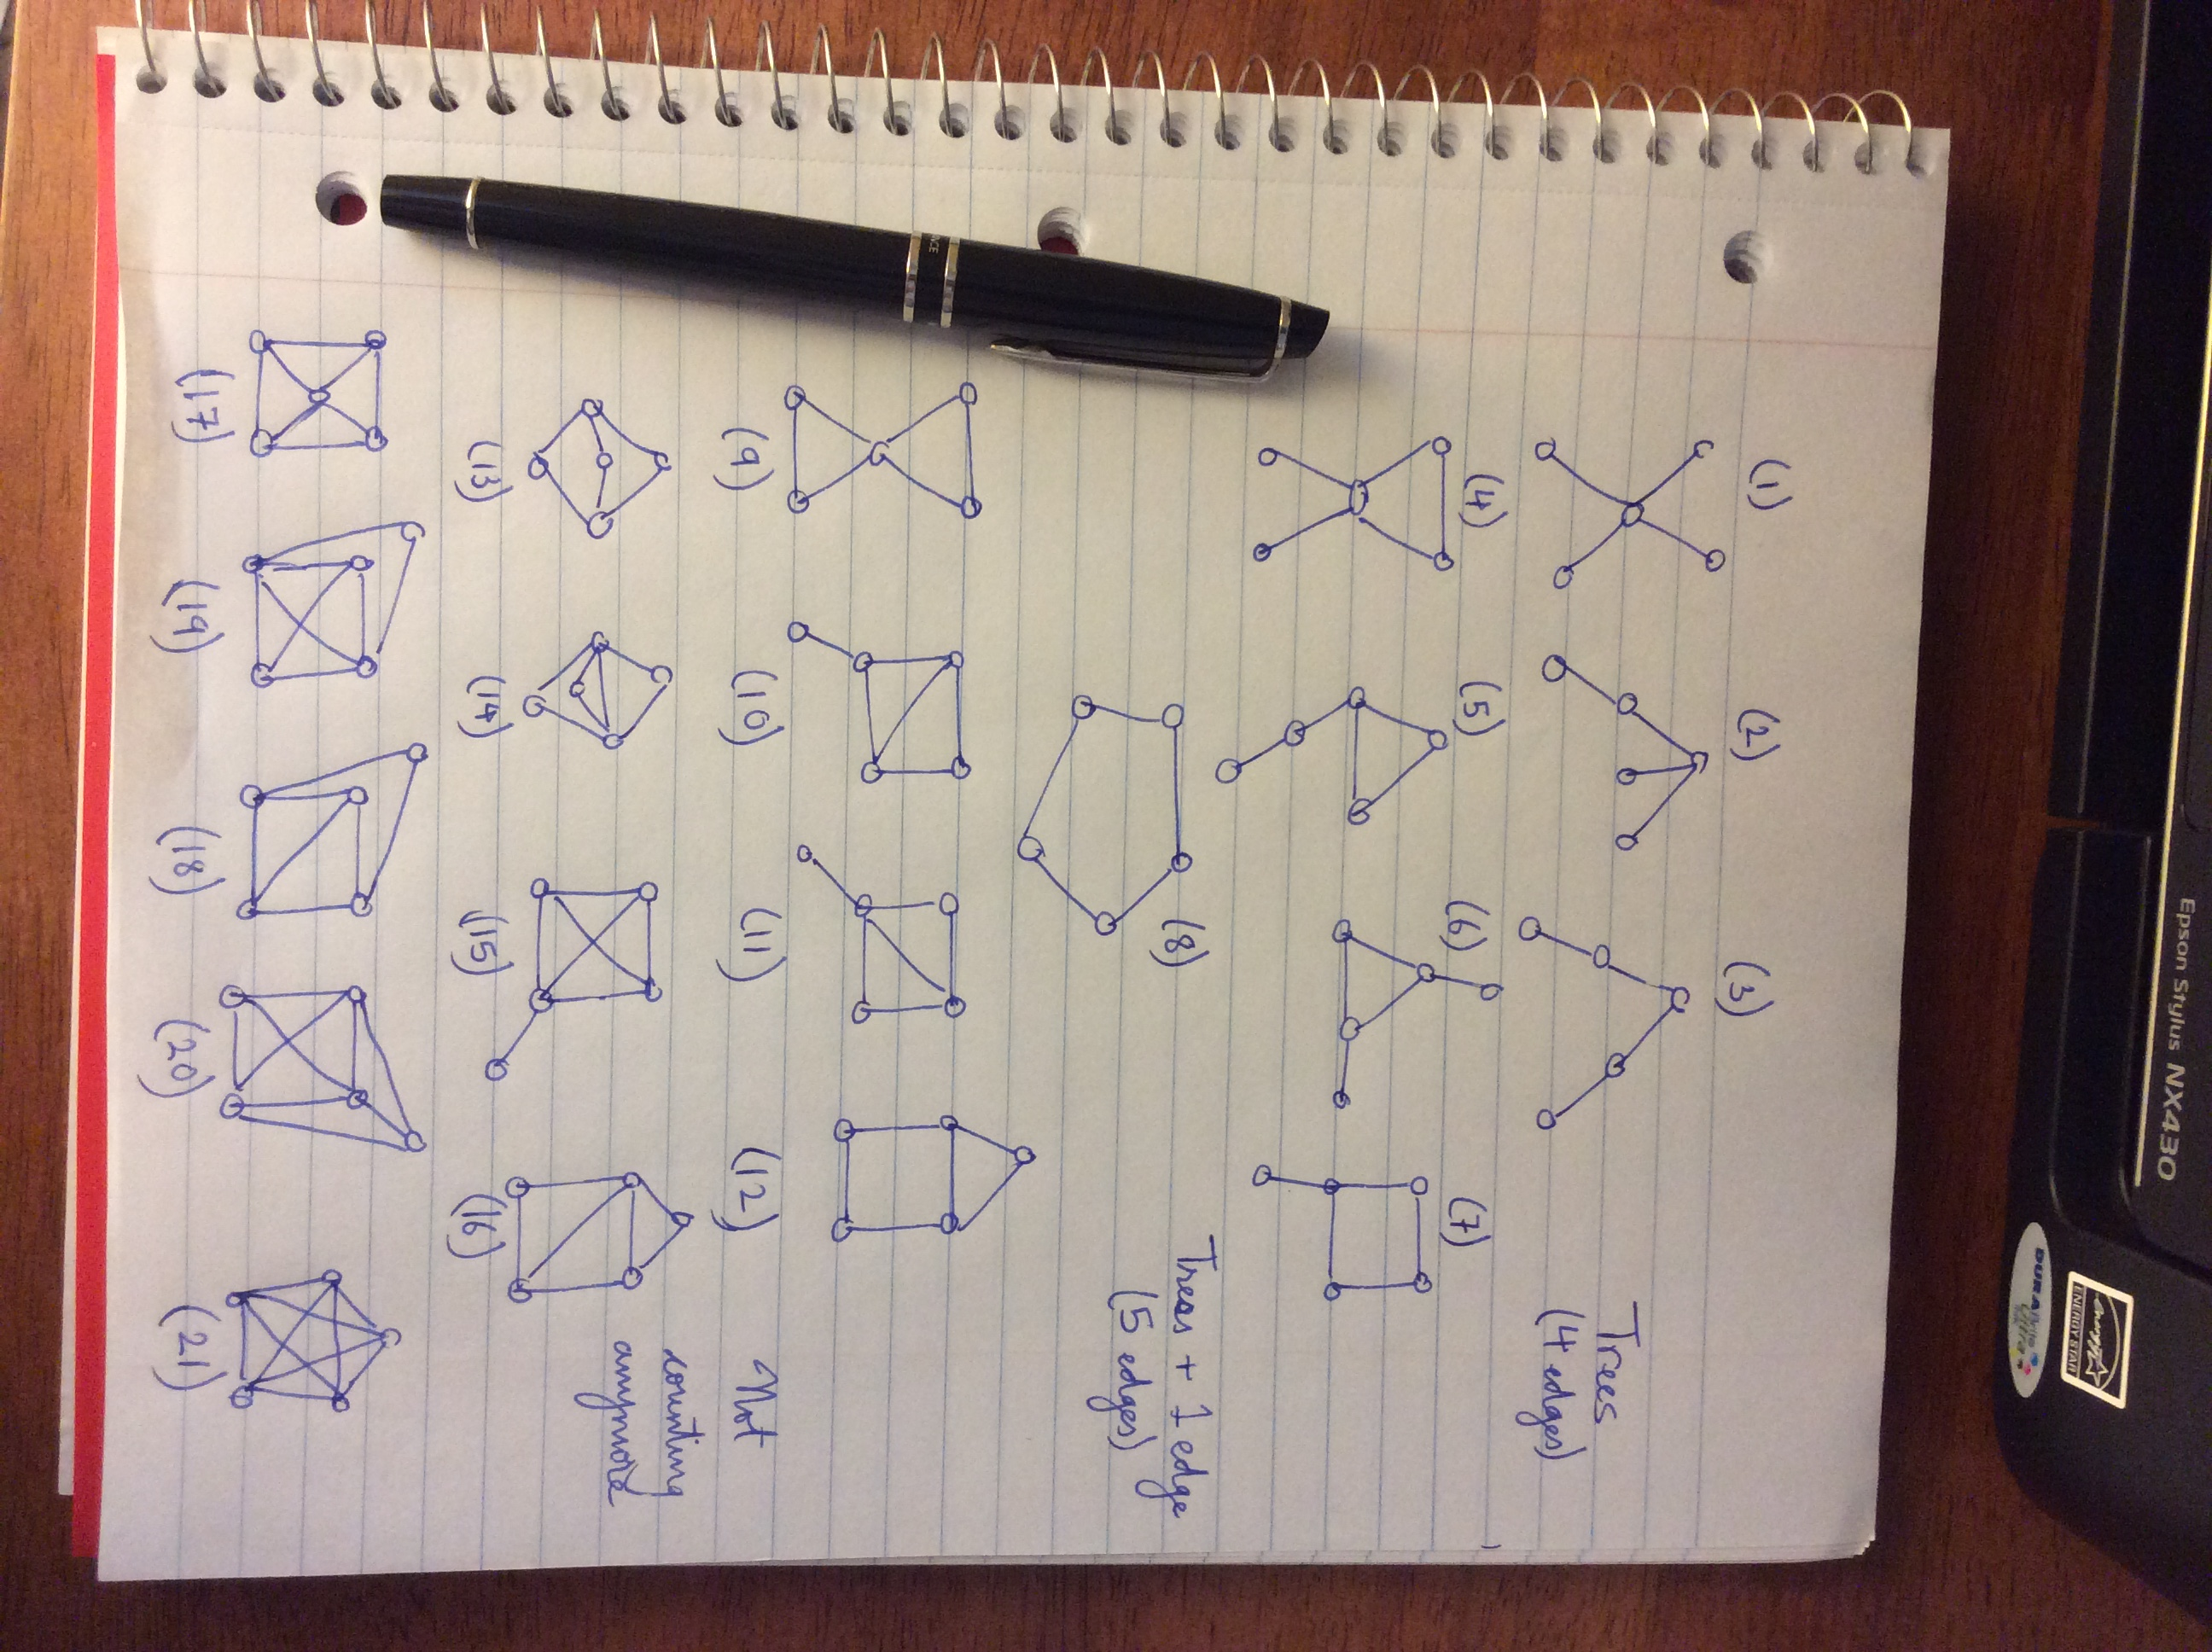
\includegraphics[angle=90,origin=c, width=1\linewidth]{5-vertex.jpg}
\caption{All connected 5-vertex patterns}
\label{fig:5patterns}
\end{center}
\end{figure}

We assume we have   done the triangle enumeration and the 4-clique enumeration.   We can load those operations.  For other 4-vertex counts, we don't necessarily do enumeration,  we are restricted to what our exact counting algorithms can do.  

\section{ Notation}
\begin{itemize}
\item $d_i$: degree of node i
\item $t_i$: number of triangles incident to node i
\item $t_{ij}$: number of  triangles incident to  edge (i,j)
\item $d^+_i=\sum_{(i,j)\in E} d_j-1$: sum of degrees of nodes incident to node i, after removing connections to i.  
\item $C^k_i:$ number of $k$-cliques vertex i   is part of. 
\item  $C^k_{ij}$: number of $k$-cliques  that edge (i,j)   is part of. 
\end{itemize} 
\section{Patterns} 
For simplicity of notation, I assume ${0\choose 2}=0$  and ${1\choose 2}=0$.

\begin{itemize} 
\item {\bf Pattern 1}
\[ \#_1=\sum_{i=1}^n {d_i \choose 4} \] 
\item{\bf Pattern 2} 
\[\#_2=\sum_{i=1}^n {d_i-1 \choose 2} d_i^+-t_i(d_i-2) \]
Here the challenge is tailed triangles,  the term $t_i(d_i-2)$ accounts  for such triangles. 
\item{\bf Pattern 3} 
\[\#_3= \sum_{i=1}^n \sum_{(i,j)\in E} \frac{(d_j-1)(d^+_i-d_j+1)}{2} -(t_{ij}*(d_j-2)) \] 
Vertex i is the top vertex, j is one of its  children. The correction term is for tailed triangles. 
\item{\bf Pattern 4} 
\[\#_4= \sum_{i=1}^n t_i {d_i-2\choose 2}  \] 
\item{\bf Pattern 5} 
\[ \#_5= \sum_i (\sum_{e_{ij}\in E} (t_i-t_{ij})(d_j-2)) -\sum_{e_{ij}\in E}{t_{ij}\choose 2}  \] 
Vertex i is the left vertex of the triangle and j  is the middle vertex of the tail.   We need to account for the last vertex of the tail connecting back to the triangle.  The corrective term  counts chorded 4-cycles where vertex i  is connected to the chord. 
\item{\bf Pattern 6} 
\[ \#_6= \sum_{e_{ij}\in E} (t_{ij}*(d_i-1)(d_j-2) -{t_{ij}\choose 2}  \] 
Here i is the top vertex of the triangle and  j is  right vertex of the triangle.  The corrective term is for chorded 4-cycles.
\item{\bf Pattern 7}
I don't know how to  write this in  closed form. But with my current 4-cycle code I can count all non-induced 4-cycles per vertex and  I will be able to add this to  that code. 
\item{\bf Pattern 8}
\item{\bf Pattern 9}
 Let vertex i be the  central vertex of the pattern,
 \[    \#_9 = \sum_{i=1}^n {t_i \choose 2} - \sum_{e_{ij}\in E } {t_{ij} \choose 2} \]
\item{\bf Pattern 10}
 We  can count this pattern by collecting some additional information  during triangle counting. Per each edge, collect the cumulative degrees  of the third vertex of the triangle this vertex participates in. We will refer to this quantity as $td_{ij}$. We also  need a corrective term  to exclude 4-cliques. 
 \[   \#_{10} = \sum_{e_{ij \in E}} (td_{ij}-2t_{ij}) *2(t_{ij} - 1) - C^4_{ii}\]
\item{\bf Pattern 11}
If e = (i,j) is the diagonal edge of the pattern, then
   \[ \#_{11}(e) = \sum_{e_{ij}\in E} (d_i+d_j - 6) * {t_{ij} \choose 2}  \] 
\item{\bf Pattern 12}
Again, I cannot   count them with my code, given triangle counts. 
\item{\bf Pattern 13}
Ali's current 4 cycles code can do this. I would be surprised if Sesh's code  cannot. 
\item{\bf Pattern 14}
 if e is the diagonal edge, then
 \[   \#_{14}= \sum_{e_{ij \in E}}  {t_{ij} \choose 3}\]
\item{\bf Pattern 15}
Extension of 4-clique counts 
\item{\bf Pattern 16}
maybe there's a better way, but here's a two-pass triangle enumeration approach.  In the first pass compute nTr(e).  In second pass, for each triangle (u, v, w), let e1 = (u, v), e2 = (u, w), e3 = (v, w).  Let t be the central triangle in the pattern:
   \[ \#_{16}(t) = (nTr(e1) - 1) * (nTr(e2) - 1) 
                     +(nTr(e1) - 1) * (nTr(e3) - 1) 
                     +(nTr(e2) - 1) * (nTr(e3) - 1)
                     - nC4(e1) - nC4(e2) - nC4(e3) \] 
    But I think that if you add all $count_16(t)$ values, the "correction" is just -12*nC4(G) (that's 12 times the number of 4-cliques). Pick a triangle in a 4-clique, and take any pair of edges. From this, we can create a distinct "false" pattern 16.
                  
                     
\item{\bf Pattern 17}
\item{\bf Pattern 18}
\item{\bf Pattern 19}
4-clique enumeration+triangle counts 
\item{\bf Pattern 20}

\item{\bf Pattern 21}
We  will  probably do clique enumeration.


\end{itemize}
\newpage
\subsection{Conversion to induced counts}
The following matrix  can be used to commute the number of induced counts from  non-induced counts. 
 Matrix entry $a_{ij}$  corresponds to how many times pattern $j$ appears  in pattern $i$ as a non-induced pattern. 
{\tiny
\[ 
\left(
\begin{array}{ccccccccccccccccccccc}
1 &  &0 &0 &0 &0 &0 &0 &0 &0 &0 &0 &0 &0 &0 &0 &0 &0 &0 &0 &0  \\
0 &1 &0 &0 &0 &0 &0 &0 &0 &0 &0 &0 &0 &0 &0 &0 &0 &0 &0 &0 &0  \\
0 &0 &1 &0 &0 &0 &0 &0 &0 &0 &0 &0 &0 &0 &0 &0 &0 &0 &0 &0 &0  \\
1 &2 &0 &1 &0 &0 &0 &0 &0 &0 &0 &0 &0 &0 &0 &0 &0 &0 &0 &0 &0  \\
0 &1 &2 &0 &1 &0 &0 &0 &0 &0 &0 &0 &0 &0 &0 &0 &0 &0 &0 &0 &0  \\
0 &2 &1 &0 &0 &1 &0 &0 &0 &0 &0 &0 &0 &0 &0 &0 &0 &0 &0 &0 &0  \\
0 &2 &2 &0 &0 &0 &1 &0 &0 &0 &0 &0 &0 &0 &0 &0 &0 &0 &0 &0 &0  \\
0 &0 &5 &0 &0 &0 &0 &1 &0 &0 &0 &0 &0 &0 &0 &0 &0 &0 &0 &0 &0  \\
1 &4 &4 &2 &4 &0 &0 &0 &1 &0 &0 &0 &0 &0 &0 &0 &0 &0 &0 &0 &0  \\
0 &4 &4 &0 &2 &2 &1 &0 &0 &1 &0 &0 &0 &0 &0 &0 &0 &0 &0 &0 &0  \\
1 &5 &2 &2 &0 &2 &1 &0 &0 &0 &1 &0 &0 &0 &0 &0 &0 &0 &0 &0 &0  \\
0 &4 &7 &0 &2 &1 &2 &1 &0 &0 &0 &1 &0 &0 &0 &0 &0 &0 &0 &0 &0  \\
0 &6 &6 &0 &0 &0 &6 &0 &0 &0 &0 &0 &1 &0 &0 &0 &0 &0 &0 &0 &0  \\
2 &12 &6 &6 &0 &6 &6 &0 &0 &0 &6 &0 &1 &1 &0 &0 &0 &0 &0 &0 &0  \\
1 &9 &6 &3 &3 &6 &3 &0 &0 &3 &3 &0 &0 &0 &1 &0 &0 &0 &0 &0 &0  \\
1 &10 &10 &3 &6 &5 &4 &1 &1 &2 &2 &2 &0 &0 &0 &1 &0 &0 &0 &0 &0  \\
%1 &20 &24 &4 &16 &12 &16 &4 &2 &8 &4 &12 &2 &0 &0 &4 &1 &4 &0 &0 &0  \\
%0 &10 &14 &0 &6 &4 &8 &2 &0 &2 &0 &4 &1 &0 &0 &0 &0 &1 &0 &0 &0  \\
%2 &20 &18 &8 &12 &14 &12 &2 &2 &8 &10 &6 &1 &1 &2 &4 &0 &1 &1 &0 &0  \\
%3 &36 &36 &15 &30 &30 &30 &6 &6 &24 &24 &24 &4 &3 &6 &15 &0 &9 &6 &1 &0  \\
%5 &60 &60 &30 &60 &60 &60 &12 &15 &60 &60 &60 &10 &10 &20 &30 &5 &30 &30 &10 &1  \\
0 &10 &14 &0 &6 &4 &8 &2 &0 &2 &0 &4 &1 &0 &0 &0 &1 &0 &0 &0 &0  \\
1 &20 &24 &4 &16 &12 &16 &4 &2 &8 &4 &12 &2 &0 &0 &4 &4 &1 &0 &0 &0  \\
2 &20 &18 &8 &12 &14 &12 &2 &2 &8 &10 &6 &1 &1 &2 &4 &1 &0 &1 &0 &0  \\
3 &36 &36 &15 &30 &30 &30 &6 &6 &24 &24 &24 &4 &3 &6 &15 &9 &0 &6 &1 &0  \\
5 &60 &60 &30 &60 &60 &60 &12 &15 &60 &60 &60 &10 &10 &20 &30 &30 &5 &30 &10 &1  
\end{array}
\right)
\]
}

Here, we remove zeros. 
{\tiny
\[ 
\left(
\begin{array}{ccccccccccccccccccccc}
1 &  &  &  &  &  &  &  &  &  &  &  &  &  &  &  &  &  &  &  &   \\
   &1 &  &  &  &  &  &  &  &  &  &  &  &  &  &  &  &  &  &  &   \\
   &  &1 &  &  &  &  &  &  &  &  &  &  &  &  &  &  &  &  &  &   \\
1 &2 &  &1 &  &  &  &  &  &  &  &  &  &  &  &  &  &  &  &  &   \\
   &1 &2 &  &1 &  &  &  &  &  &  &  &  &  &  &  &  &  &  &  &   \\
&2 &1 &  &  &1 &  &  &  &  &  &  &  &  &  &  &  &  & & &  \\
 &2 &2 &  &  &  &1 &  &  &  &  &  &  &  &  &  &  &  &  &  &   \\
 &  &5 &  &  &  &  &1 &  &  &  &  &  &  &  &  &  &  &  &  &   \\
1 &4 &4 &2 &4 &  &  &  &1 &  &  &  &  &  &  &  &  &  &  &  &   \\
 &4 &4 &  &2 &2 &1 &  &  &1 &  &  &  &  &  &  &  &  &  &  &   \\
1 &5 &2 &2 &  &2 &1 &  &  &  &1 &  &  &  &  &  &  &  &  &  &   \\
 &4 &7 &  &2 &1 &2 &1 &  &  &  &1 &  &  &  &  &  &  &  &  &   \\
 &6 &6 &  &  &  &6 &  &  &  &  &  &1 &  &  &  &  &  &  &  &   \\
2 &12 &6 &6 &  &6 &6 &  &  &  &6 &  &1 &1 &  &  &  &  &  &  &   \\
1 &9 &6 &3 &3 &6 &3 &  &  &3 &3 &  &  &  &1 &  &  &  &  &  &   \\
1 &10 &10 &3 &6 &5 &4 &1 &1 &2 &2 &2 &  &  &  &1 &  &  &  &  &   \\
%&10 &14 &  &6 &4 &8 &2 &  &2 &  &4 &1 &  &  &  &1  & &  &  &   \\
%1 &20 &24 &4 &16 &12 &16 &4 &2 &8 &4 &12 &2 &  &  &4 &4 &1 &  &  &   \\
%2 &20 &18 &8 &12 &14 &12 &2 &2 &8 &10 &6 &1 &1 &2 &4 &1  &1 & &  &   \\
%3 &36 &36 &15 &30 &30 &30 &6 &6 &24 &24 &24 &4 &3 &6 &15 &9  & &6 &1 &   \\
%5 &60 &60 &30 &60 &60 &60 &12 &15 &60 &60 &60 &10 &10 &20 &30 &305 &5 &30 &10 &1  
 &10 &14 &  &6 &4 &8 &2 &  &2 &  &4 &1 &  &  &  &1 &  &  &  &   \\
1 &20 &24 &4 &16 &12 &16 &4 &2 &8 &4 &12 &2 &  &  &4 &4 &1 &  &  &   \\
2 &20 &18 &8 &12 &14 &12 &2 &2 &8 &10 &6 &1 &1 &2 &4 &1 &  &1 &  &   \\
3 &36 &36 &15 &30 &30 &30 &6 &6 &24 &24 &24 &4 &3 &6 &15 &9 &  &6 &1 &   \\
5 &60 &60 &30 &60 &60 &60 &12 &15 &60 &60 &60 &10 &10 &20 &30 &30 &5 &30 &10 &1  
\end{array}
\right)
\]
}
The transpose  of this matrix is
{\tiny
\[ 
\left(
\begin{array}{ccccccccccccccccccccc}

1& & & 1& & & & & 1& & 1& & & 2& 1& 1& & 1& 2& 3& 5 \\
& 1& & 2& 1& 2& 2& & 4& 4& 5& 4& 6& 12& 9& 10& 10& 20& 20& 36& 60 \\
& & 1& & 2& 1& 2& 5& 4& 4& 2& 7& 6& 6& 6& 10& 14& 24& 18& 36& 60 \\
& & & 1& & & & & 2& & 2& & & 6& 3& 3& & 4& 8& 15& 30 \\
& & & & 1& & & & 4& 2& & 2& & & 3& 6& 6& 16& 12& 30& 60 \\
& & & & & 1& & & & 2& 2& 1& & 6& 6& 5& 4& 12& 14& 30& 60 \\
& & & & & & 1& & & 1& 1& 2& 6& 6& 3& 4& 8& 16& 12& 30& 60 \\
& & & & & & & 1& & & & 1& & & & 1& 2& 4& 2& 6& 12 \\
& & & & & & & & 1& & & & & & & 1& & 2& 2& 6& 15 \\
& & & & & & & & & 1& & & & & 3& 2& 2& 8& 8& 24& 60 \\
& & & & & & & & & & 1& & & 6& 3& 2& & 4& 10& 24& 60 \\
& & & & & & & & & & & 1& & & & 2& 4& 12& 6& 24& 60 \\
& & & & & & & & & & & & 1& 1& & & 1& 2& 1& 4& 10 \\
& & & & & & & & & & & & & 1& & & & & 1& 3& 10 \\
& & & & & & & & & & & & & & 1& & & & 2& 6& 20 \\
& & & & & & & & & & & & & & & 1& & 4& 4& 15& 30 \\
& & & & & & & & & & & & & & & & 1& 4& 1& 9& 30 \\
& & & & & & & & & & & & & & & & & 1& & & 5 \\
& & & & & & & & & & & & & & & & & & 1& 6& 30 \\
& & & & & & & & & & & & & & & & & & & 1& 10 \\
& & & & & & & & & & & & & & & & & & & & 1 \\
\end{array}
\right)
\]
}

The inverse of the transpose matrix is
{\tiny
\[ 
\left(
\begin{array}{rrrrrrrrrrrrrrrrrrrrr}
1& & & -1& & & & & 1& & 1& & & -2& -1& -1& & 1& 2& -3& -15 \\
& 1& & -2& -1& -2& -2& & 4& 4& 5& 4& 6& -12& -9& -10& -10& 20& 20& -6& -340 \\
& & 1& & -2& -1& -2& -5& 4& 4& 2& 7& 6& -6& -6& -10& -14& 24& 18& 6& -420 \\
& & & 1& & & & & -2& & -2& & & 6& 3& 3& & -4& -8& 12& 50 \\
& & & & 1& & & & -4& -2& & -2& & & 3& 6& 6& -16& -12& & 260 \\
& & & & & 1& & & & -2& -2& -1& & 6& 6& 5& 4& -12& -14& 9& 180 \\
& & & & & & 1& & & -1& -1& -2& -6& 6& 3& 4& 8& -16& -12& -6& 260 \\
& & & & & & & 1& & & & -1& & & & 1& 2& -4& -2& -3& 68 \\
& & & & & & & & 1& & & & & & & -1& & 2& 2& -3& -25 \\
& & & & & & & & & 1& & & & & -3& -2& -2& 8& 8& -6& -100 \\
& & & & & & & & & & 1& & & -6& -3& -2& & 4& 10& -18& -20 \\
& & & & & & & & & & & 1& & & & -2& -4& 12& 6& 6& -180 \\
& & & & & & & & & & & & 1& -1& & & -1& 2& 1& 2& -30 \\
& & & & & & & & & & & & & 1& & & & & -1& 3& -10 \\
& & & & & & & & & & & & & & 1& & & & -2& 6& -20 \\
& & & & & & & & & & & & & & & 1& & -4& -4& 9& 20 \\
& & & & & & & & & & & & & & & & 1& -4& -1& -3& 50 \\
& & & & & & & & & & & & & & & & & 1& & & -5 \\
& & & & & & & & & & & & & & & & & & 1& -6& 30 \\
& & & & & & & & & & & & & & & & & & & 1& -10 \\
& & & & & & & & & & & & & & & & & & & & 1 \\
\end{array}
\right)
\]
}
\end{document}
